% 32-07(32쪽) — 증가하는 함수 y=f(x) 의 그래프와 직선 y=x, a·b·c·d 를 잇는 안내 점선. 스캔 화질이 낮아 TikZ 로 다시 그림.
% 원문에 있는 것만 옮긴다: 곡선 · 직선 y=x · x축·y축에 평행한 점선 · 라벨 O, x, y, a, b, c, d, y=f(x), y=x. 눈금값은 원문에 없다.
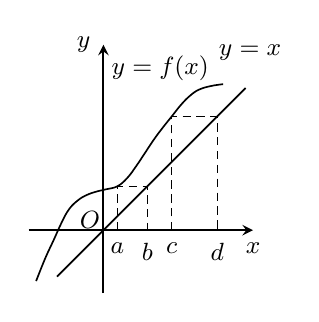
\begin{tikzpicture}[x=0.38cm, y=0.38cm, line width=0.6pt]
  \draw[->, >=stealth, line width=0.7pt] (-2.5,0) -- (5.0,0) node[below=1pt, font=\small] {$x$};
  \draw[->, >=stealth, line width=0.7pt] (0,-2.1) -- (0,6.2) node[left=1pt, font=\small] {$y$};
  \draw[densely dashed, line width=0.4pt] (0.47,0) -- (0.47,1.47) -- (1.47,1.47) -- (1.47,0);
  \draw[densely dashed, line width=0.4pt] (2.28,0) -- (2.28,3.80) -- (3.80,3.80) -- (3.80,0);
  \draw[line width=0.6pt] (-1.55,-1.55) -- (4.75,4.75);
  \draw plot[smooth, tension=0.7] coordinates {(-2.25,-1.7) (-1.95,-0.95) (-1.65,-0.30) (-1.40,0.25) (-1.15,0.70) (-0.85,1.00) (-0.55,1.18) (-0.20,1.30) (0.10,1.37) (0.47,1.47) (0.8,1.75) (1.1,2.15) (1.4,2.60) (1.7,3.05) (2.0,3.45) (2.28,3.80) (2.6,4.20) (2.9,4.50) (3.2,4.70) (3.6,4.82) (4.0,4.88)};
  \node[font=\small] at (-0.45,0.33) {$\pt{O}$};
  \node[below=1pt, font=\small] at (0.47,0) {$a$};
  \node[below=1pt, font=\small] at (1.47,0) {$b$};
  \node[below=1pt, font=\small] at (2.28,0) {$c$};
  \node[below=1pt, font=\small] at (3.80,0) {$d$};
  \node[font=\small] at (1.9,5.4) {$y=f(x)$};
  \node[font=\small] at (4.9,5.95) {$y=x$};
\end{tikzpicture}
